\documentclass{beamer}
%\documentclass[handout,t]{beamer}

\batchmode
% \usepackage{pgfpages}
% \pgfpagesuselayout{4 on 1}[letterpaper,landscape,border shrink=5mm]

\usepackage{ctex,amsmath,amssymb,enumerate,epsfig,bbm,calc,color,ifthen,capt-of}
\usepackage{url} 
\usepackage{hyperref} 

\usetheme{Berlin}
%\usecolortheme{mit}

\title{媒体云转码的演进:\\\Small{MapReduce、DASH与稳定婚姻}}
\author{Alan Zhuang\\
\href{mailto:cheedoong@acm.org}{\nolinkurl{cheedoong@acm.org}}\\
}
\date{\today}
\pgfdeclareimage[height=0.25cm]{mit-logo}{tencent_alpha.png}
\logo{\pgfuseimage{mit-logo}\hspace*{0.1cm}}

\AtBeginSection[]
{
\begin{frame}<beamer>
\frametitle{Outline}
\tableofcontents[currentsection]
\end{frame}
}
\beamerdefaultoverlayspecification{<+->}
% -----------------------------------------------------------------------------
\begin{document}
% -----------------------------------------------------------------------------

\frame{\titlepage}

\section[Outline]{}
\begin{frame}{Outline}
\tableofcontents
\end{frame}

% -----------------------------------------------------------------------------
\section{背景}
\begin{frame}{多屏时代的挑战}
\begin{itemize}
\pause
\item 多种平台\\ \pause
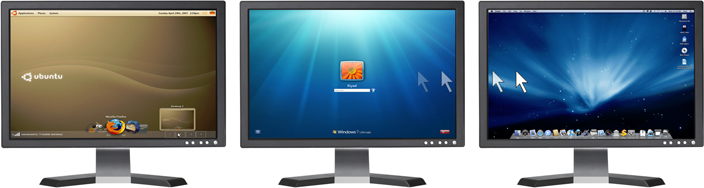
\includegraphics[height=1.6cm]{fig/PCs.png}\hspace*{0.1cm}\pause
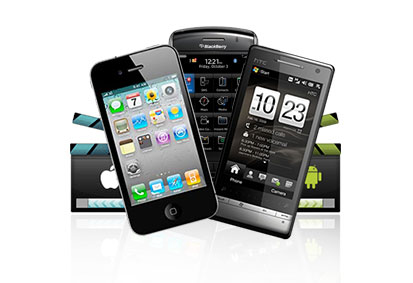
\includegraphics[height=1.6cm]{fig/mobile-bc.png}\hspace*{0.1cm}\pause
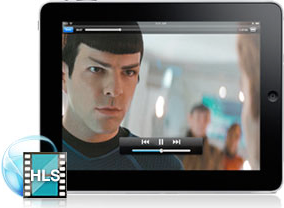
\includegraphics[height=1.6cm]{fig/streaming-bc.png}
\item 多种屏幕大小\\ \pause
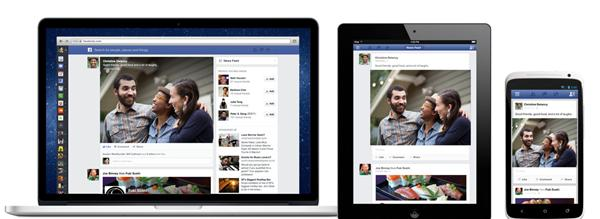
\includegraphics[height=1.2cm]{fig/screen_sizes.jpg}\hspace*{0.1cm}\pause
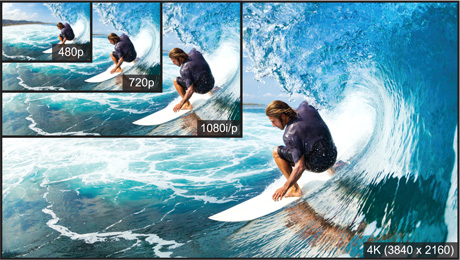
\includegraphics[height=2cm]{fig/480_to_4KVideo.jpg}\hspace*{0.1cm}\pause
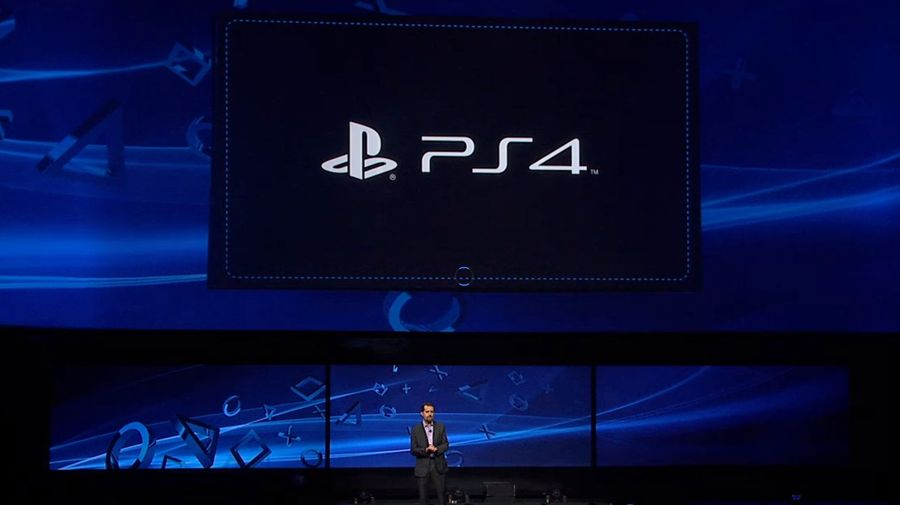
\includegraphics[height=2cm]{fig/4k_video.jpg}
\end{itemize}
\end{frame}
\begin{frame}{多屏时代的挑战} 
\begin{itemize}  
\pause
\item 多种码率\\ 
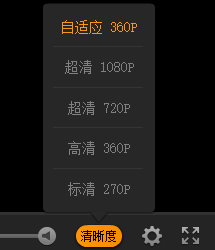
\includegraphics[height=2cm]{fig/bitrate_tencent.png}\hspace*{0.1cm}\pause
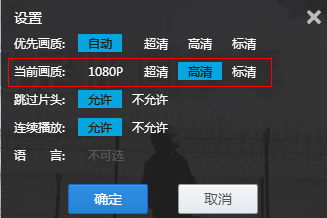
\includegraphics[height=2cm]{fig/bitrate_youku.png}\hspace*{0.1cm}\pause
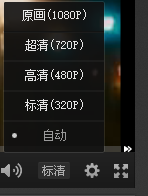
\includegraphics[height=2cm]{fig/bitrate_sohu.png}\hspace*{0.1cm}\pause
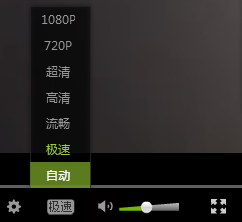
\includegraphics[height=2cm]{fig/bitrate_qiyi.png}\pause   
\item 多种解码能力\\ 
%\begin{table}
{\scriptsize
\begin{center}
\begin{tabular}{l|llll} %\toprule
\hline
联发科芯片& MT6572 & MT6582 & MT6588 & MT6592 \\ %\midrule
\hline
Display  & 960$\times$540P & 1280$\times$720P & 1920$\times$1280P & 1920$\times$1280P \\
H.264 Decode   & 720P@30fps & 1080P@30fps  & 1080P@30fps  & 1080P@30fps \\ 
HEVC Decode   &  N/A &  N/A  & 720P@30fps  & 720P@30fps \\ 
\hline
%\bottomrule
\end{tabular}
}
\end{center}
%\end{table}
\pause
\item 多种封装容器支持\\
\item 多种编码标准支持\\

\item 巨头角力\\
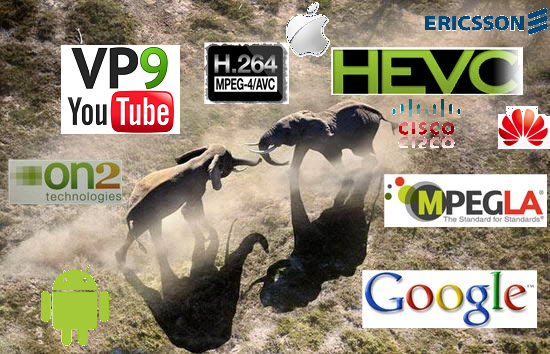
\includegraphics[height=3cm]{fig/competition.png}\pause
\end{itemize}
\end{frame}
\begin{frame}{目标与约束}
\begin{itemize}
\item 十一假期基本完成
\item 回来后合并
\item alan: 总体,关键算法
\item roshan: 统领协调整理,后台架构设计
\item xiaojun, edge: 整理以往代码,补充
\item michael: 搜索相关,自然语言理解
\item molly: 后勤,其他
\end{itemize}
\end{frame}
\begin{frame}{目标与约束}
\includegraphics[scale=0.38]{fig/team7.jpg}
\end{frame}
\begin{frame}{工欲善其事,必先利其器}
What 利器?
\pause
\begin{itemize}
\item \LaTeX{} with a patent template
\item Evernote \&QQMail
\item Dropbox \& WeiYun
\item ACM Digital Library \url{http://dl.acm.org}
\item SOOPAT \url{http://soopat.com} 
\item Google Patents \url{http://patents.google.com}
\item BibTeX to manage the references
\end{itemize}
\end{frame}
\begin{frame}{整体架构}

\end{frame}
\begin{frame}{投影拟合}

\end{frame}
\begin{frame}{投影拟合}

\end{frame}
\begin{frame}{投影拟合}
\begin{itemize}
\item 好不容易弄到一张符合要求的矢量地图
\item 发现该地图所采用的投影方法和高斯-克吕格尔投影、Lambert投影都有些接近
\item 但无论怎么调整参数,总存在稍许旋转、拉伸和扭曲
\end{itemize}
\pause 准确坐标和近似投影的坐标的关系:\pause 
\begin{itemize}
	\item 若仅有平移差别,那么x,y分别只是m\_x,m\_y的线性函数
	\item 若仅有两个方向上的拉伸,则$x = f(m\_x); y = g(m\_y)$
	\item 若存在旋转变换,甚至非仿射变换,则$x = f(m\_x, m\_y); y = g(m\_x, m\_y)$
\end{itemize}
\end{frame}
\begin{frame}{投影拟合}
\begin{center}

\end{center}
The RBF model is
\begin{equation}
f(x)=\sum_{i=1}^n \alpha_i g(\norm{x-x_i}).
\end{equation}
The output is a linear combination of non-linear functions of the input.  The non-linearity is a function of distance only.
\end{frame}
\begin{frame}{RBF neutral network}
An RBF is the solution to the following interpolation problem:
\begin{equation}
\min \sum_{i=1}^n L(f(x_i),y_i) + \lambda \norm{f}_H.
\end{equation}
\begin{equation}
\min \: \norm{f}_H \quad\text{st.}\quad f(x_i)=y_i, \quad i=1,2,...,n.
\end{equation}

This is similar to a kernel density, except that the coefficients $\alpha_i$ are not restricted to a convex combination, and the basis function $g$ does not have to be a density.
\end{frame}
\begin{frame}  
\begin{equation}
E = 1/2 \sum_i \int (y(x_i+z)-y_i)^2 p(z) dz
\end{equation}
Let
\begin{equation}
f(x) = y(x) + \eta(x)
\end{equation}
\begin{align}
E(f) & = 1/2 \sum_i \int (y(x_i+z) + \eta(x_i+z) - y_i)^2 p(z) dz \\
& \approx 1/2 \sum_i \int (y(x_i+z) - y_i)^2 + 2(y(x_i+z)+\eta(x_i+z)-y_i)\eta(x_i+z) p(z) dz \\
\end{align}
\begin{equation}
\delta E = \sum_i \int (y(x_i+z)-y_i)\eta(x_i+z) p(z) dz = 0
\end{equation}
\end{frame}
\begin{frame}
Let $\eta(x)=\delta(x-u)$.
\begin{align}
\delta E & = \sum_i \int (y(x_i+z)-y_i)\delta(x_i+z-u) p(z) dz \\
& = \sum_i (y(u)-y_i) p(u-x_i) = 0\\
y(u)\sum_i p(u-x_i) & = \sum_i y_i p(u-x_i) \\
y(u) & = \sum_i y_i \frac{p(u-x_i)}{\sum_j p(u-x_j)}
\end{align}
\end{frame}
\begin{frame}
\pause 
近似投影:$\forall Proj_k, k \in \{1, 2, \ldots, P\}$\\
\pause 
基于曲率的角点检测,得到:\\
$(x_{ik}, y_{ik}), i \in \{1, 2, \ldots, M_k\},  k \in \{1, 2, \ldots, P\}$\\
\pause 
取相同数目$N$个对应角点,目标:
\begin{equation}
\arg \min \sum_{i=1}^{N}{[(x_i - x_{ik})^2 + (y_i - y_{ik})^2]}, k \in \{1, 2, \ldots, P\}
\end{equation}
\pause 
注意:
别人用RBF NN来做插值/拟合、分类器,而我们用它来消除误差,得到了很高的精度\\
Trial-and-error: 10+ times
\end{frame}
\begin{frame}{地址匹配与规整}

\end{frame}
\begin{frame}{地址状态机}

\end{frame}
\begin{frame}{IP库合并}

\pause 存储:一级Hash Array;二级一阶KD-Tree。\pause 考虑事实:
\begin{enumerate}
\item 拥有完整A类地址段的单位只有AT\&T、IBM、MIT;
\item 同一地域的IP段往往正好是一个完整的B类或C类地址(更精确地讲是一段内的所有IP高2或3字节相同)。
\end{enumerate}
\end{frame}
\begin{frame}{日志分析}

\end{frame}
\begin{frame}{前端处理---偏移分布}

\end{frame}
\begin{frame}{Acknowledgement}
\begin{itemize}
\item  Some of the ideas were from: 

“腾讯星云”团队
\item  Thanks for insightful discussions with: 

Nicholas Li
\item Library Support from: 

Sergey Anatolyevich Bochkanov (Russia)
\end{itemize}
\end{frame}

% -----------------------------------------------------------------------------
\section{腾讯研究院Transcoder}
\subsection{Cloud Transcoding Reusing Idle Computing Resources}
\begin{frame}{Distributed Transcoding on MapReduce}
Gale Huang, Zhenhua Li, et al. Cloud transcoder: bridging the format and resolution gap between internet videos and mobile devices. ACM NOSSDAV 2012. 
\textbf{
\includegraphics[scale=0.40]{fig/cloud_transcoder_nossdav_affiliation.png}}



\end{frame}
\begin{frame}
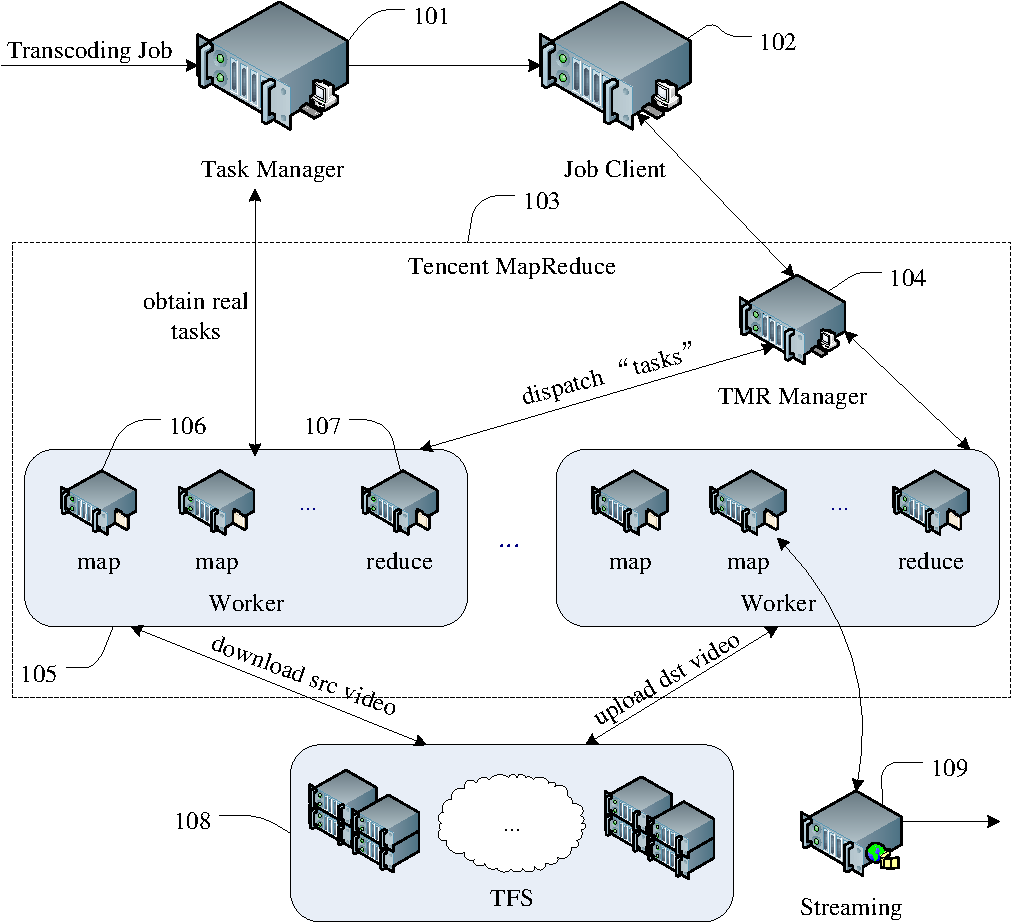
\includegraphics[scale=0.33]{fig/总体方案.pdf}\hspace*{0.1cm}
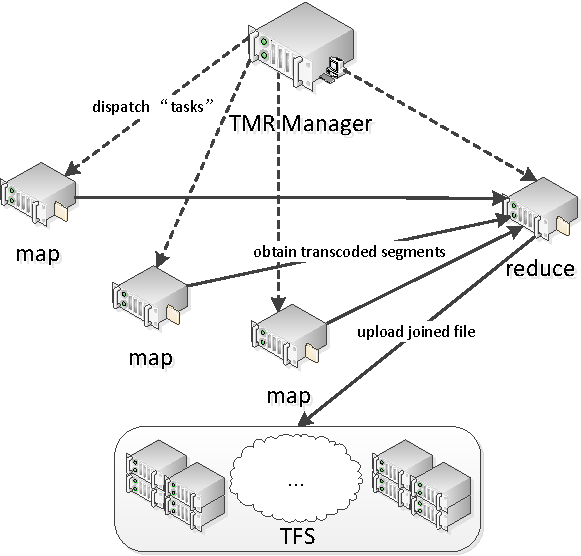
\includegraphics[scale=0.44]{fig/reduce.pdf}
\end{frame}

\begin{frame}{Distributed Transcoding on MapReduce}
\begin{center}
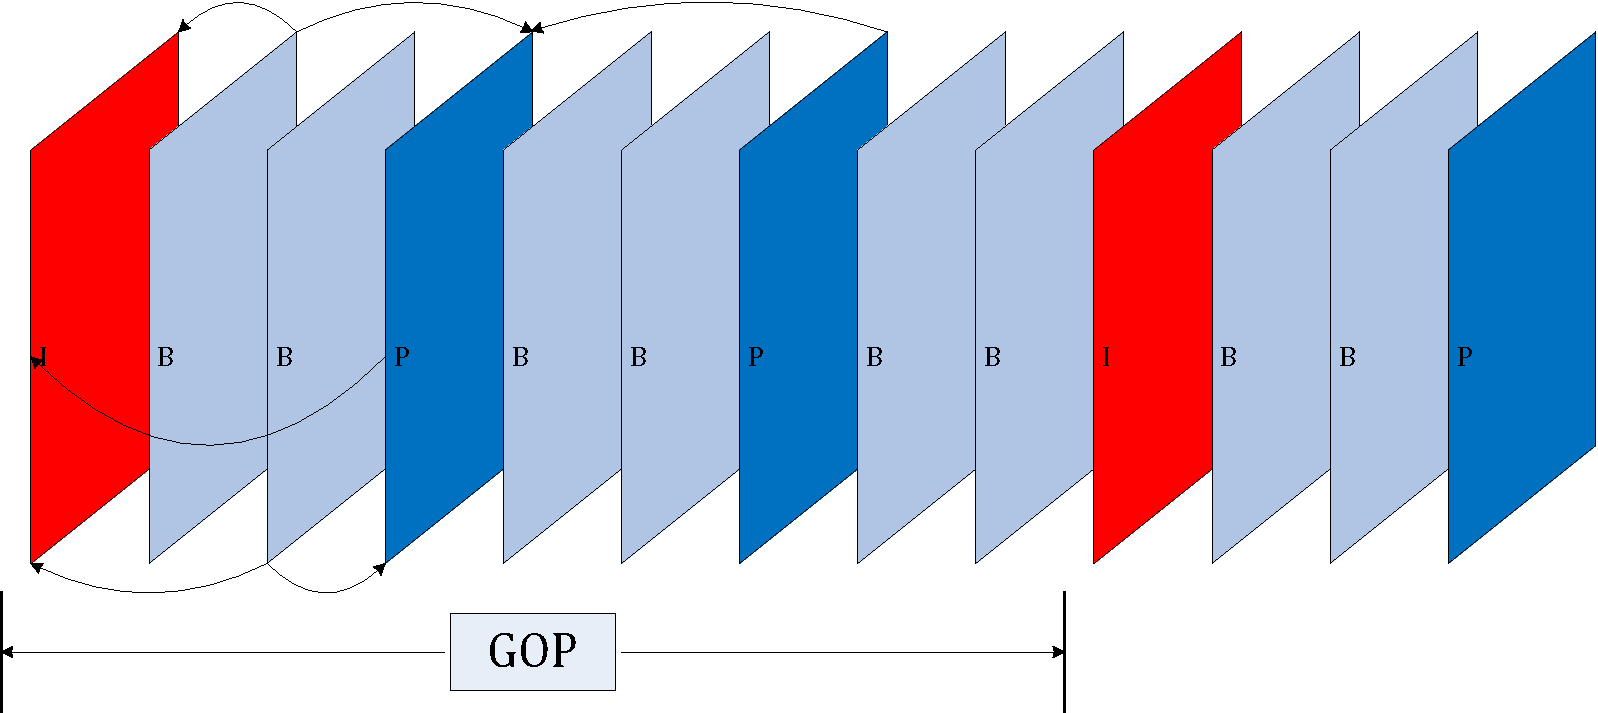
\includegraphics[scale=0.22]{fig/GOP.pdf}
\end{center}
\begin{itemize}
\item GOP-level parallelism without REAL splitting
\item Job/Map/Thread, accurate control and CPU \& I/O limitation
\item Real-time support for DASH and Live Broadcasting
\item Migration from Computing to Storage: soul of cloud tech
\item It later supported WeChat and part of Tencent Video
\end{itemize}
\end{frame}

\subsection{Fast Traversal, Scanning and Deletion on Common Disk FS; Fast Replacement on CDN Edge Nodes without Indexes}
\begin{frame}{Traversal}
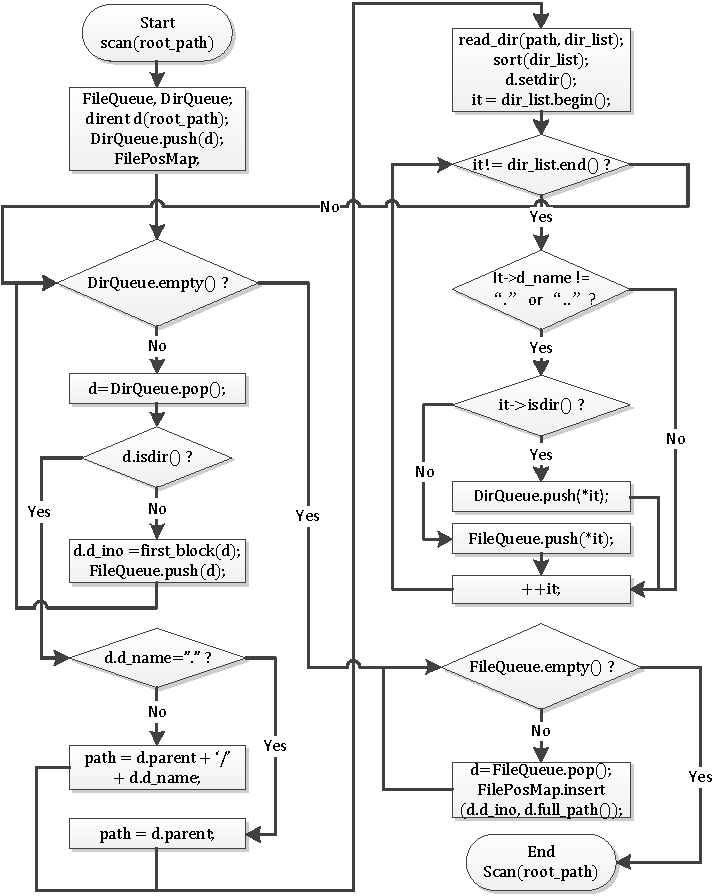
\includegraphics[scale=0.4]{fig/fs_traversal.pdf}\hspace*{0.1cm}
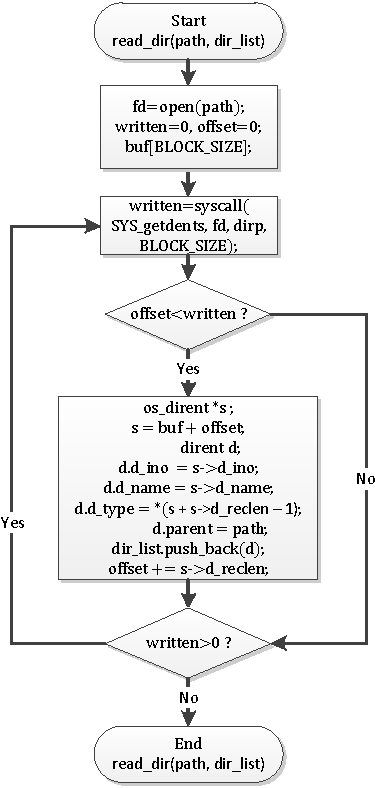
\includegraphics[scale=0.38]{fig/read_dir.pdf}\hspace*{0.1cm}
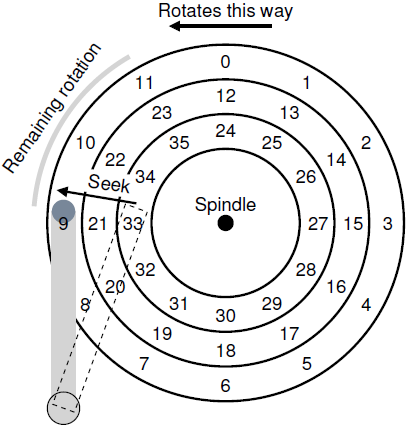
\includegraphics[scale=0.3]{fig/seek_rotate.png}
\end{frame}

%\subsection{}
\begin{frame}{Power-Law(Zip'f) Distribution}
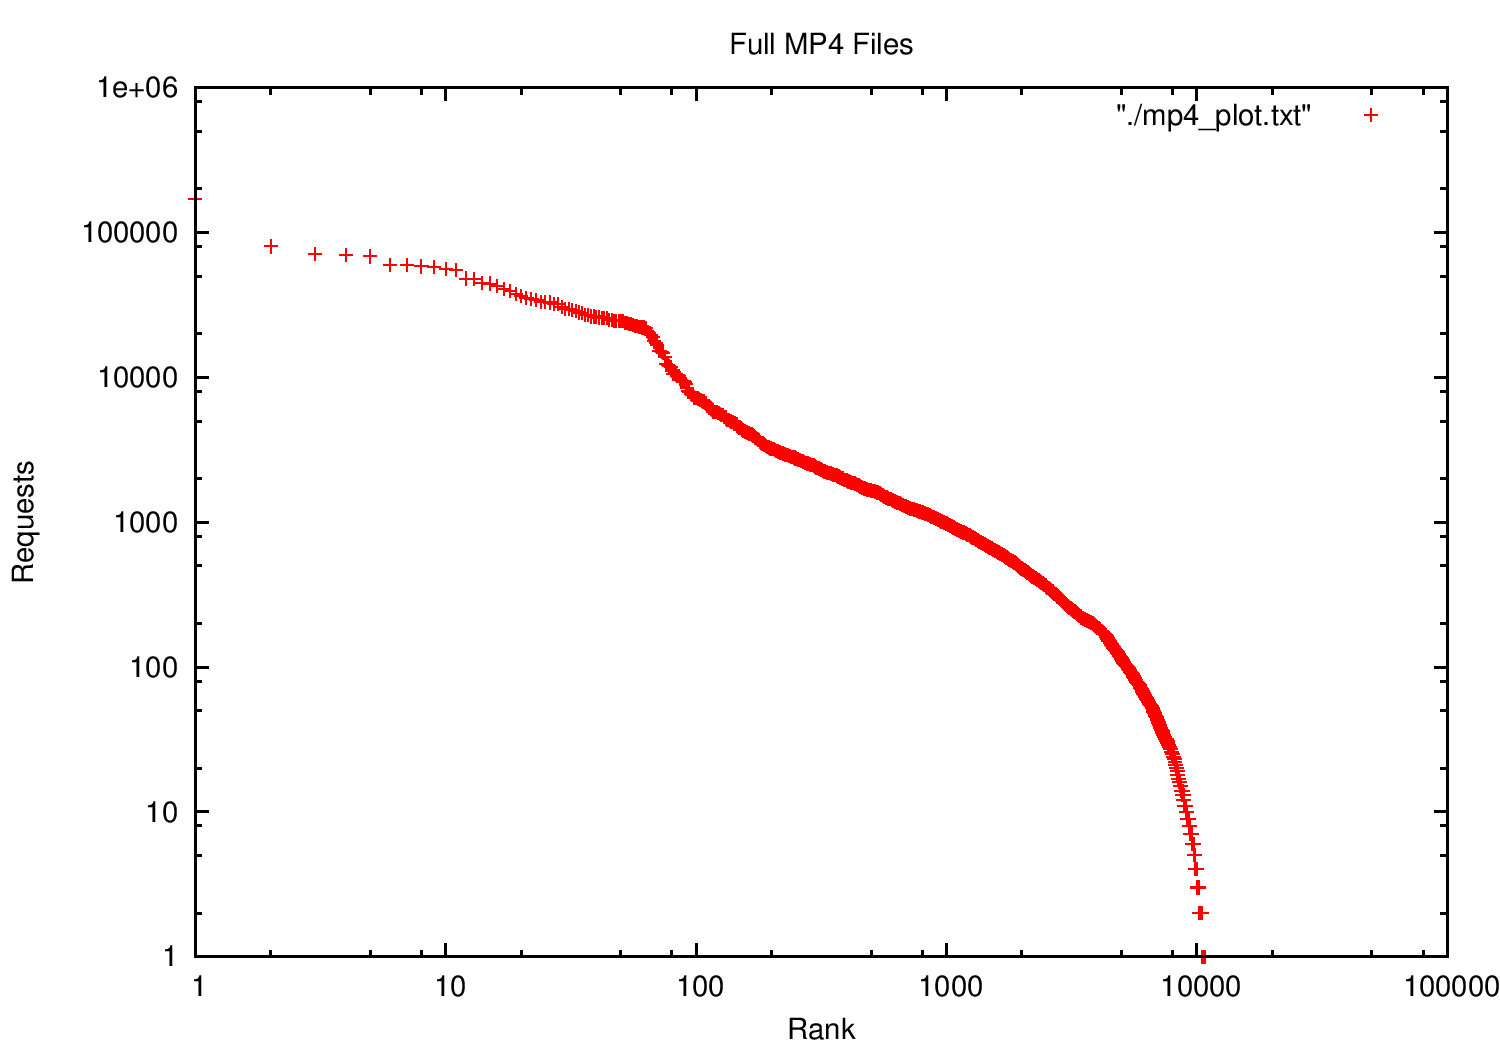
\includegraphics[scale=0.4]{fig/mp4.png}\hspace*{0.1cm}
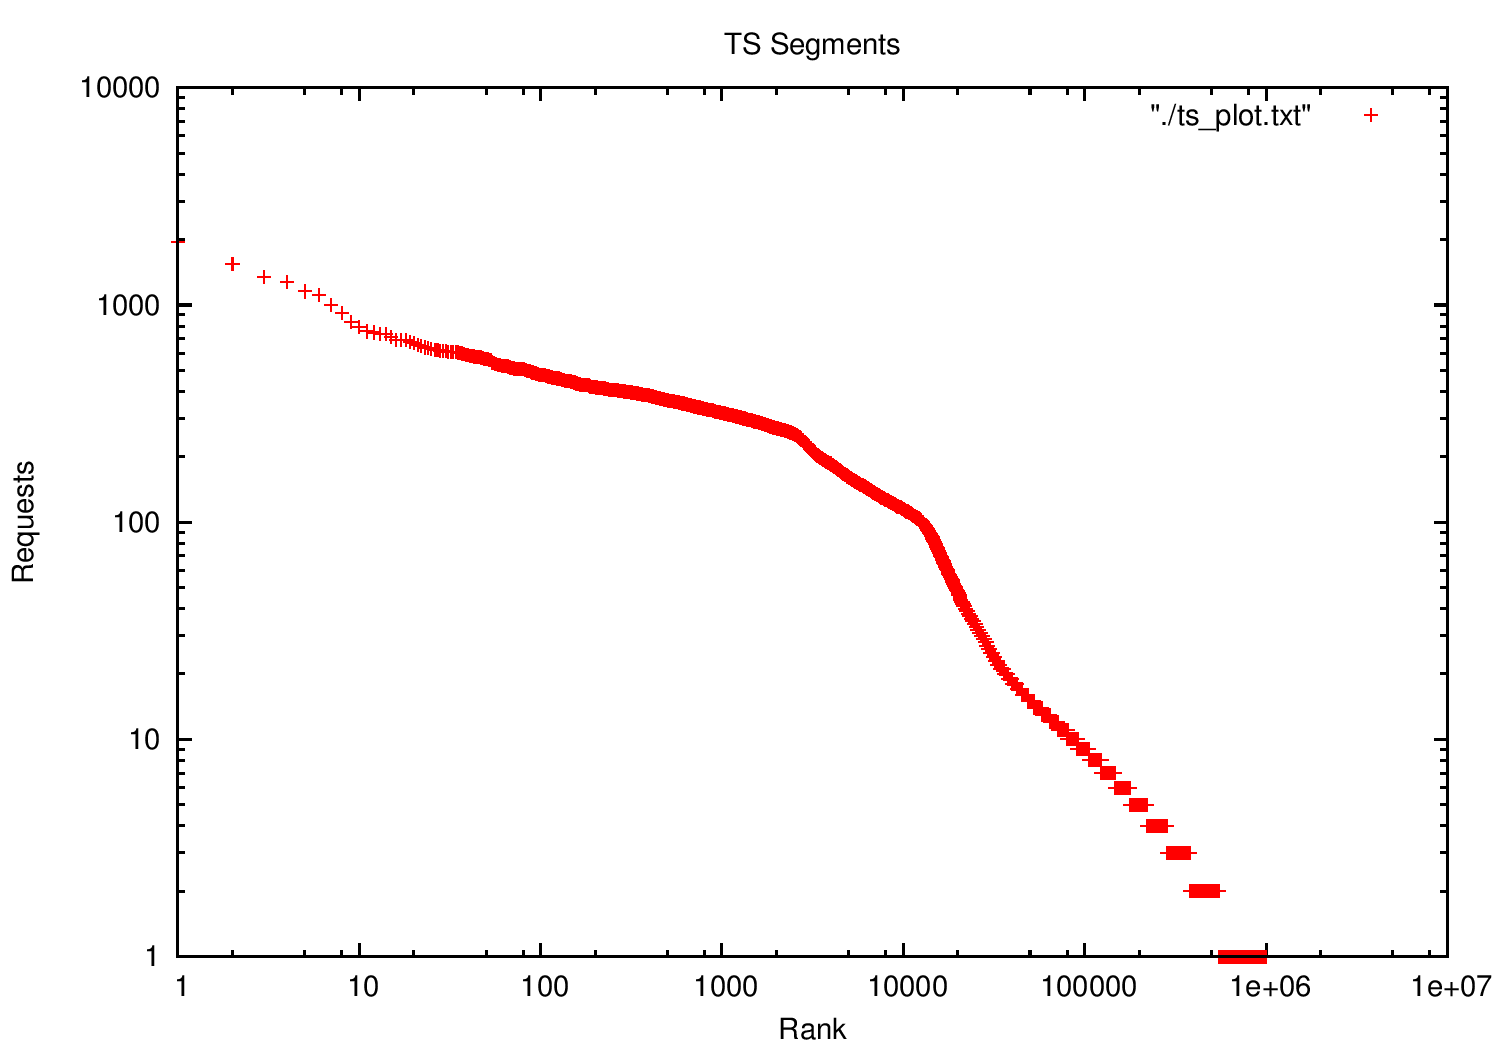
\includegraphics[scale=0.4]{fig/ts.png}
\end{frame}
\begin{frame}{Cumulative Distribution Function (CDF)}
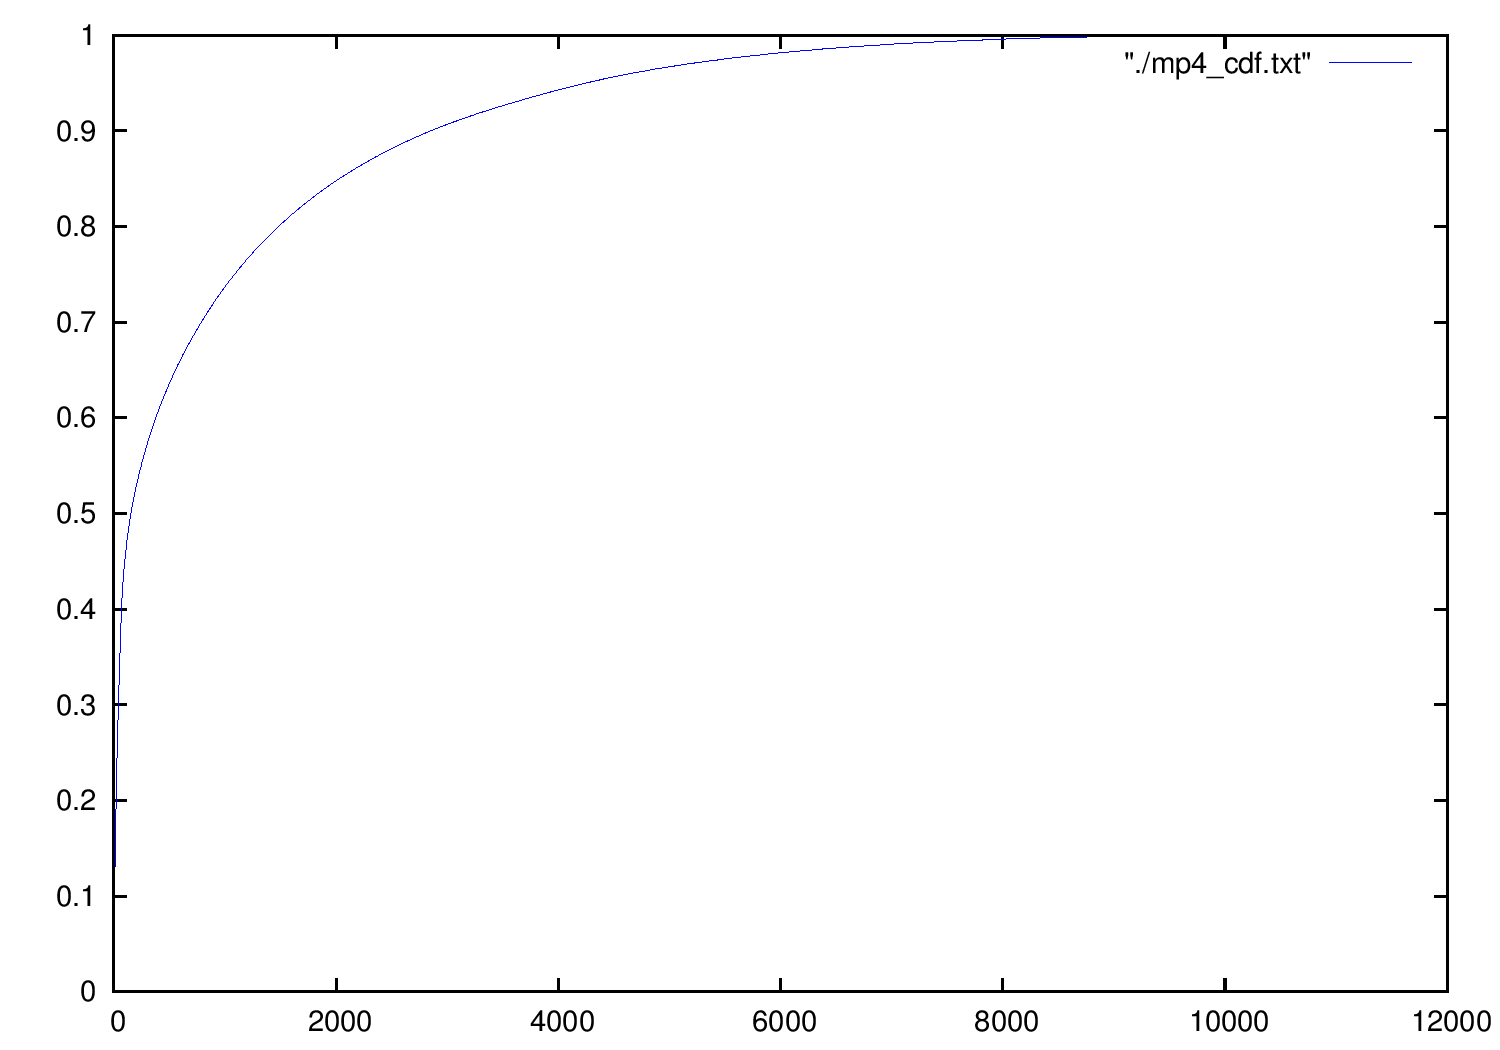
\includegraphics[scale=0.4]{fig/mp4_cdf.png}\hspace*{0.1cm}
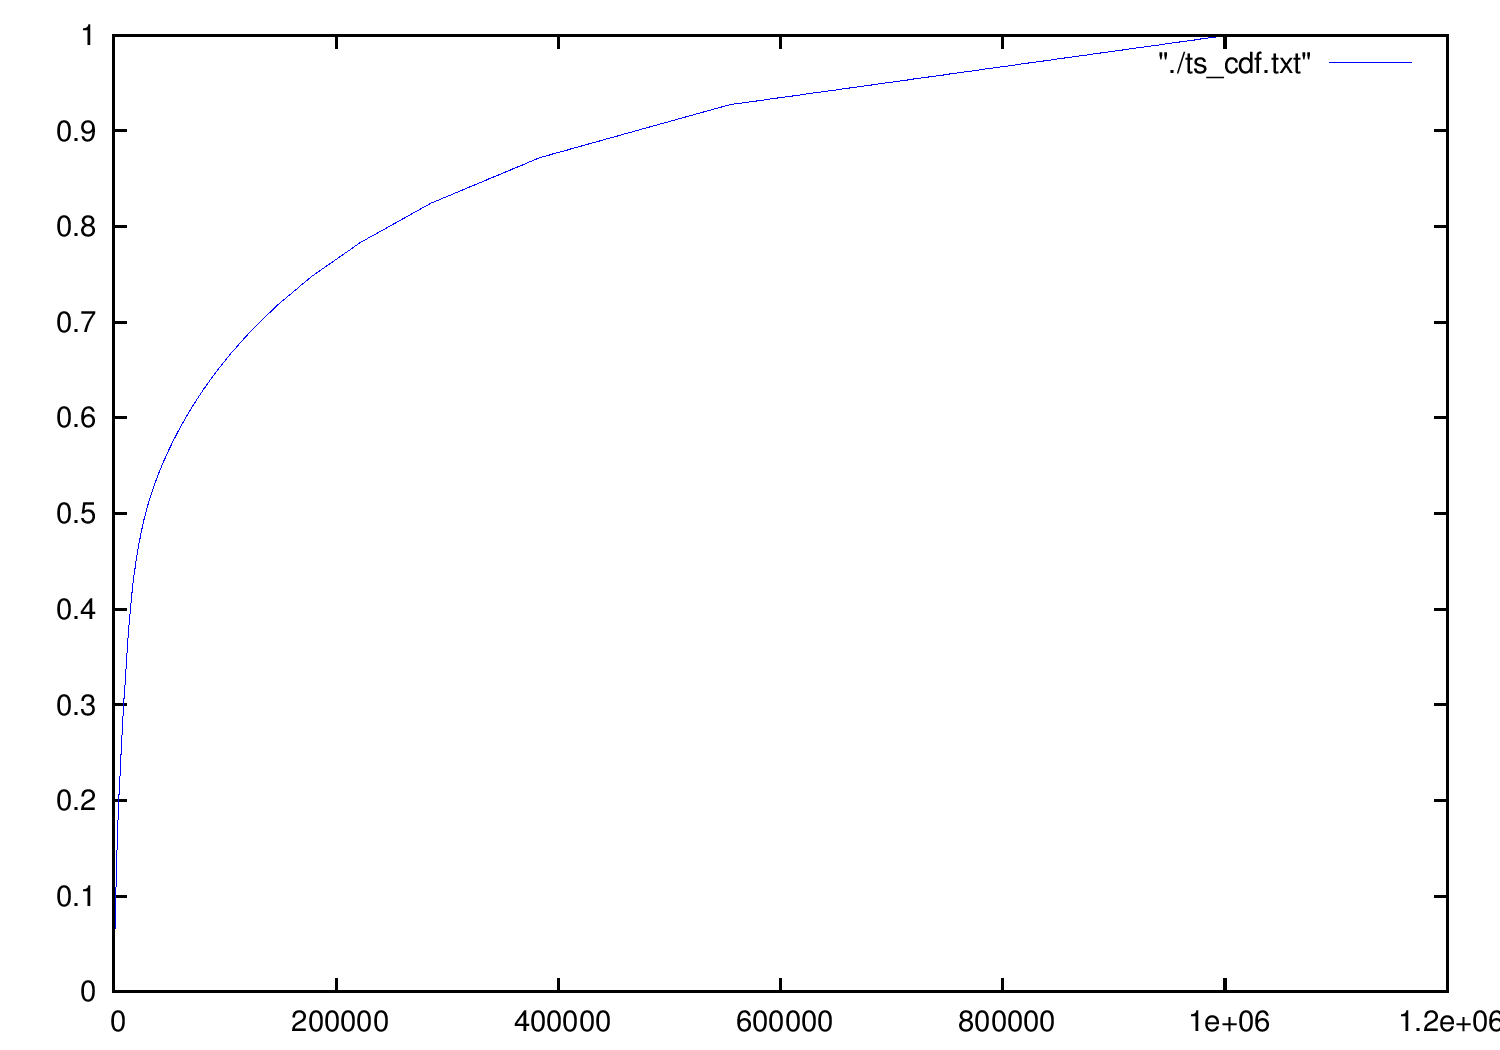
\includegraphics[scale=0.4]{fig/ts_cdf.png}
\end{frame}
\begin{frame}{Distance and ...}
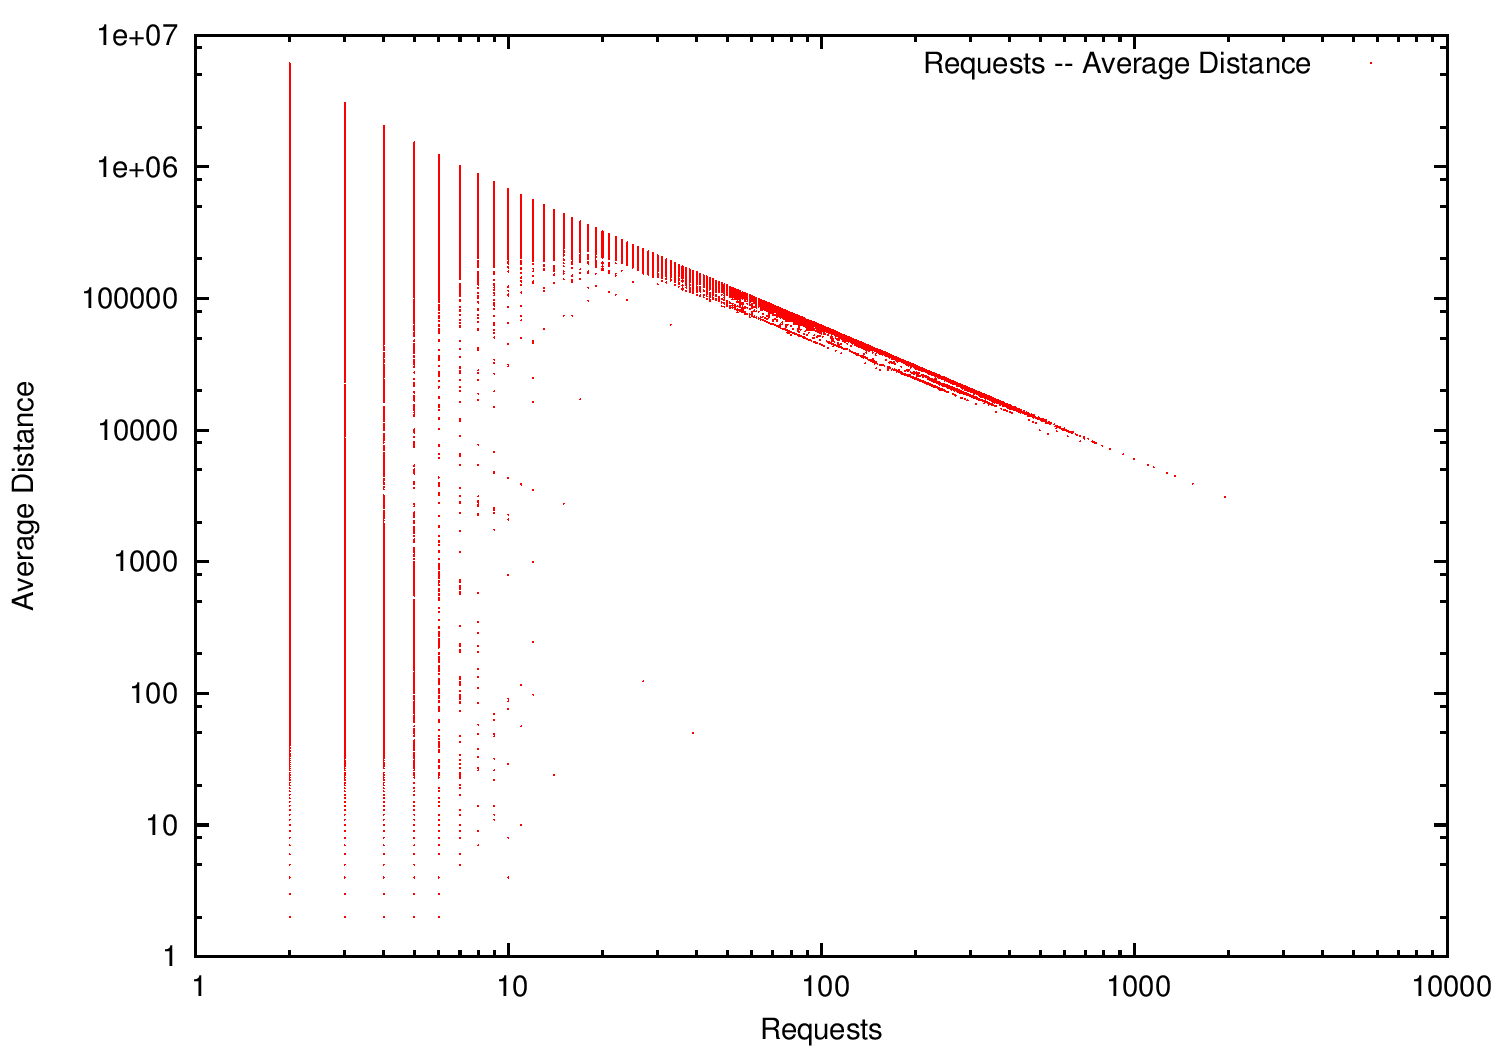
\includegraphics[scale=0.4]{fig/freq_dist.png}\hspace*{0.1cm}
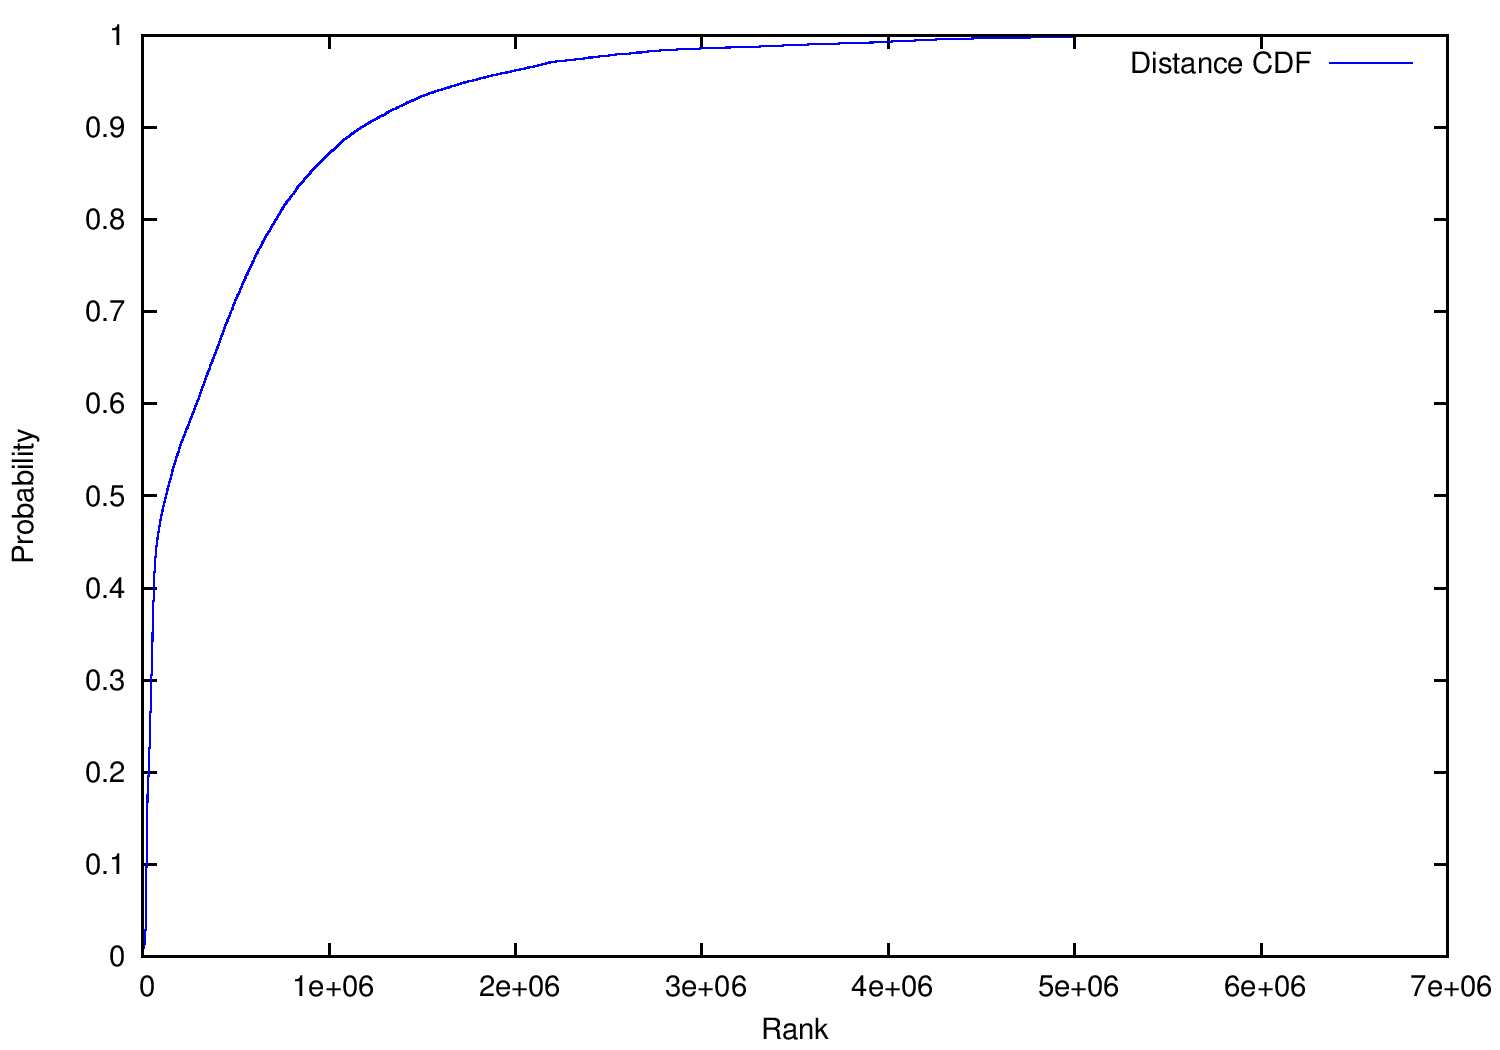
\includegraphics[scale=0.4]{fig/distance_cdf.png}
\end{frame}
\begin{frame}{i to i+1}
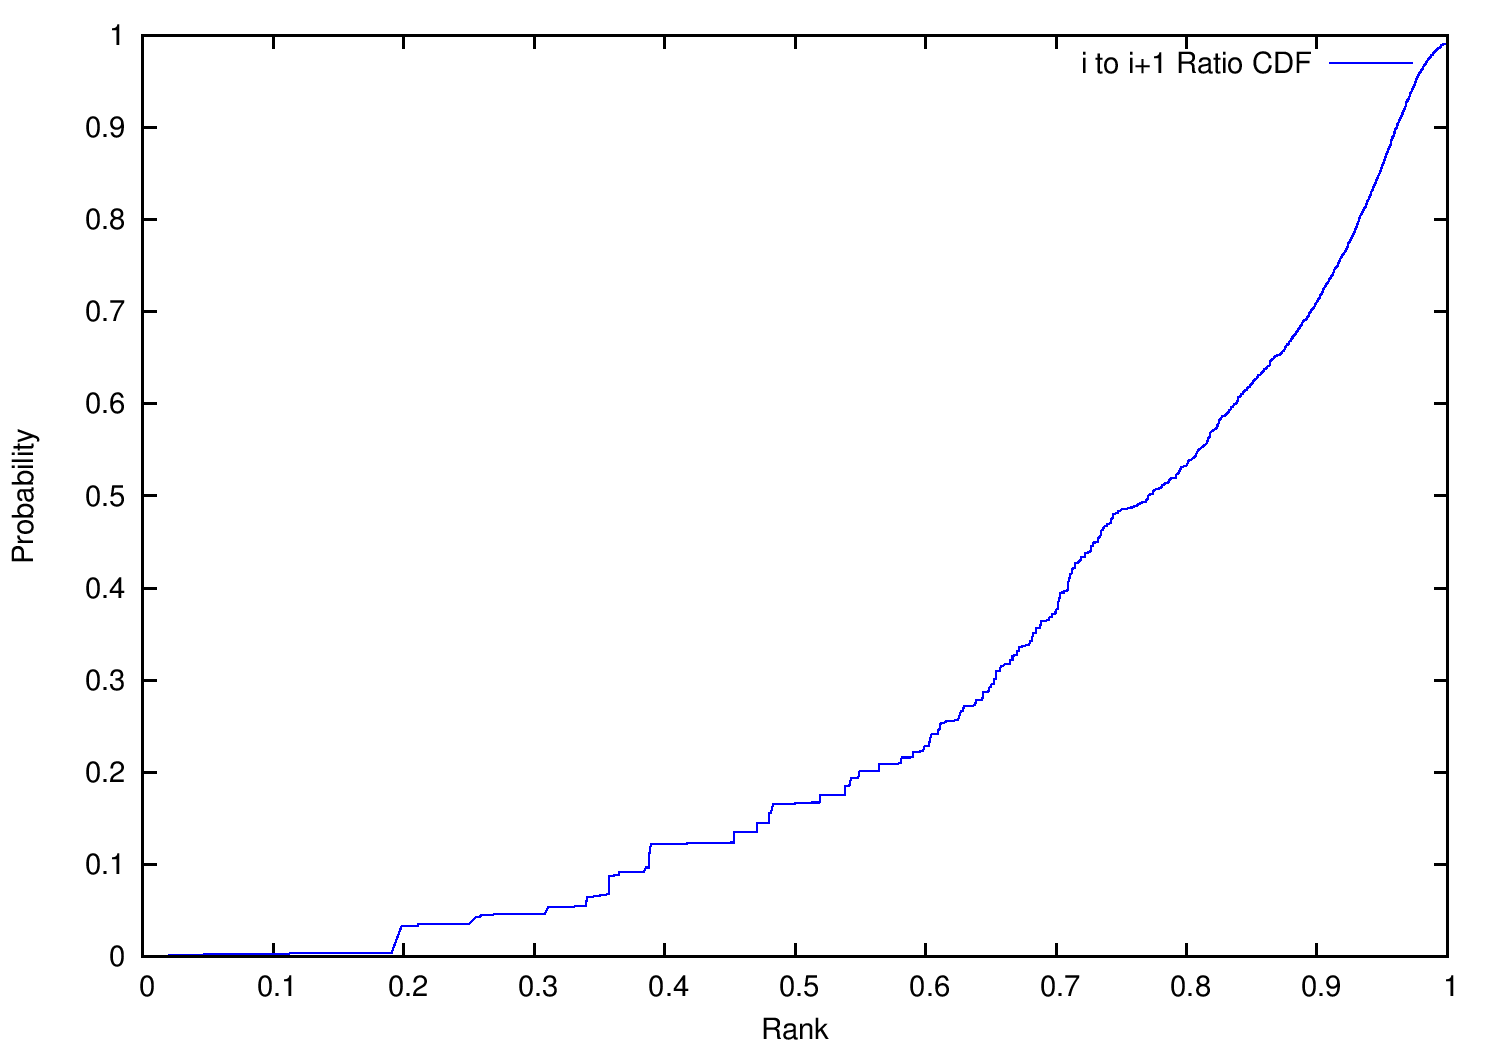
\includegraphics[scale=0.67]{fig/i_to_next_ratio_cdf.png}
\end{frame}
\begin{frame}{One of the Effects}
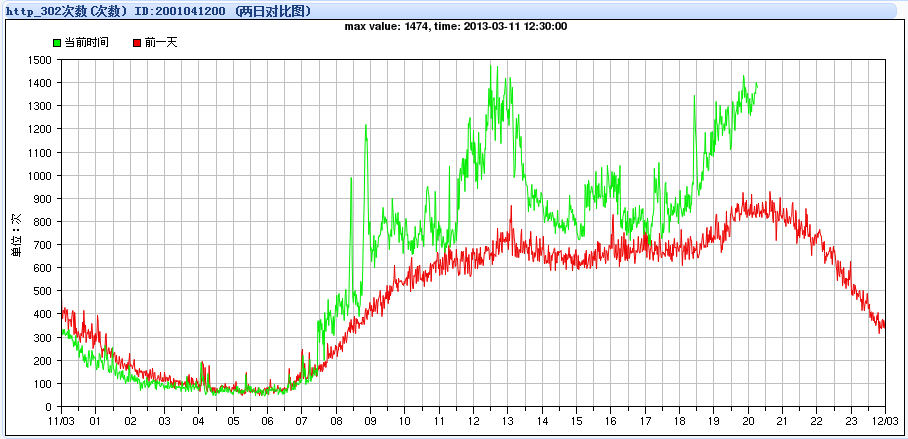
\includegraphics[scale=0.4]{fig/back_src_news.png}
\end{frame}
\begin{frame}{One of the Effects}
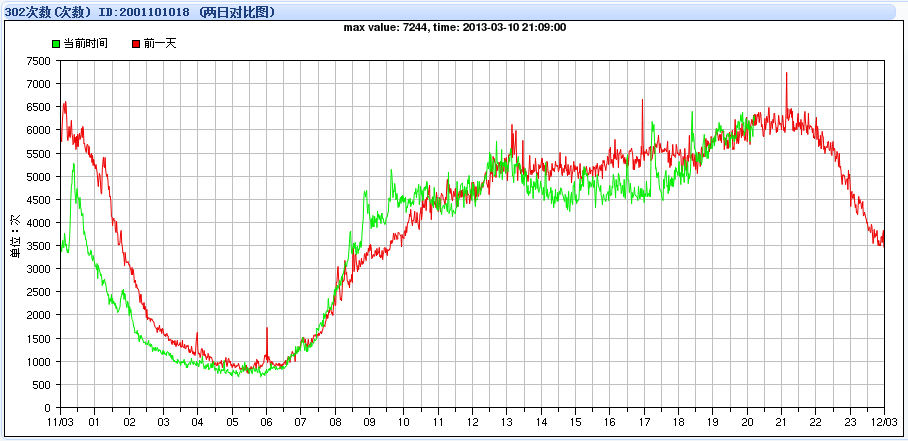
\includegraphics[scale=0.4]{fig/back_src_all.png}
\end{frame}

\section{Conclusions \& Experience}
\subsection{How to obtain new ideas?}
\begin{frame}{How to obtain new ideas?}
While working...
\pause
\begin{itemize}
\item Think more,多想
\item Try more,勇于尝试,经得起多次失败
\item Retrieve more,避免闭门造车,侧重别人没做过或做得不好的方面
\item Teamwork,每个人都有自己擅长的领域+臭皮匠理论
\end{itemize}

\end{frame}

\subsection{How to write good patent applications?}
\begin{frame}{How to write good patent applications?}
Something look like paradoxes...
\pause 
\begin{itemize}
\item 数理逻辑和推理不能够成为专利

但有一些数理支持会为专利增色不少
\item 纯粹的算法不能够成为专利

但结合具体问题、设备的算法往往能够成为高质量的专利
\item 专利不需要数据测量和效果数据

但详尽的数据测量会提供方法论上的支持,而效果数据则会提供更强的意义支撑
\end{itemize}
\end{frame}

\begin{frame}{How to write good patent applications?}
\begin{itemize}
\item 发明专利必须具有新颖性的内容,该技术领域中具有中等知识的人所不能演绎出的创造性步骤

但现在这个时代,真正具有创新性的东西太少了。所谓创新无非是:用新方法解决旧问题;或用其他领域的非新方法解决新问题。
所以就要求人涉猎广泛、融会贯通。
\item 我们显然没有足够的时间来撰写专利

但一个自我感觉良好的专利需要至少一个月的业余时间
\end{itemize}
\end{frame}
% -----------------------------------------------------------------------------
\end{document}
